\documentclass[a4paper,11pt]{jsbook}

\newcommand{\V}[1]{\boldsymbol{#1}}
\def\thline{\noalign{\hrule height 1pt}}
\def\tvline{\vrule width 1pt}

\usepackage{here} %図の場所の指定で[H](ここに貼る)を指定するためのパッケージ
\usepackage{makeidx}
\usepackage{amsmath}
\usepackage{amssymb}
\usepackage[dvipdfmx]{graphicx} %dvipdfmxはjpgやpngの張り込みのために使用

\makeindex

\pagenumbering{roman}

\begin{document}
% 表紙
\title{令和 3 年度 卒業論文\\
ロボットの内部情報を可視化する\\
ARアプリケーション}

\author{中村颯太 \\
Chiba Institute of Technology}

\date{2022年2月x日}

\maketitle

%%% 但し書き等 %%%
%この論文は、読んだあと自動的に消滅する。
%\clearpage

%%% 献辞 %%%
% D論、あるいは誰かを亡くしたときの卒論、修論等で
% 配偶者や配偶者の予定となる人の名前は覚悟をもって書くこと
%\thispagestyle{empty}
%\vfil
%\ \\
%\vspace{15em}
%\begin{center}
%	{\Large 最愛の京成線に捧ぐ }
%\end{center}
% 献辞をかかない場合はここまでコメントアウト

\include{preface}

\tableofcontents

%\cleardoublepage

%%% 本文 %%%
% 章のページの先頭は左側(奇数ページ)に来る

\cleardoublepage
\pagenumbering{arabic}

\chapter{序論}

\section{背景}
自律移動ロボットの基本的な技術の1つに自己位置推定という技術がある。
自己位置推定とは、ロボットなどがセンサー等を用いて得た情報から自身の位置や向きを推定する問題や技術を指す
%@@@句読点は???

自己位置推定の研究ではデバッグや評価のときに自律移動ロボットの内部情報と現実空間の比較が必要である。
なぜなら、ロボットが推定した自己位置を示すパーティクルの変化の観察や、
自己位置を推定に用いるセンサーから得たデータが正しく取得できているかを調べる作業は研究を行う上で重要であるためである。
%@@@「必要である→重要である」は稚拙。
%@@@ちょっとこの2文は表現が硬いかなー。もっとひらたく。あと、読点すくないような気がする。
しかし、ロボットの内部情報は数値データであるため、それだけを見て、現実空間との比較を行うことは困難である。


そのため、デバッグや評価をするには、ロボットを制御しているPCからRvizなどの可視化ツールを使用して内部情報を確認しなければならない。
%@@@この文には主語がない。句もだらだらつながっていて、どこで切って読めばいいのか曖昧。
図\ref{Rviz}はRvizで内部情報を可視化した様子である。
%@@@図の説明は?コレ見せられて読者はどうすりゃいいの?

\begin{figure}[H]
	\begin{center}
		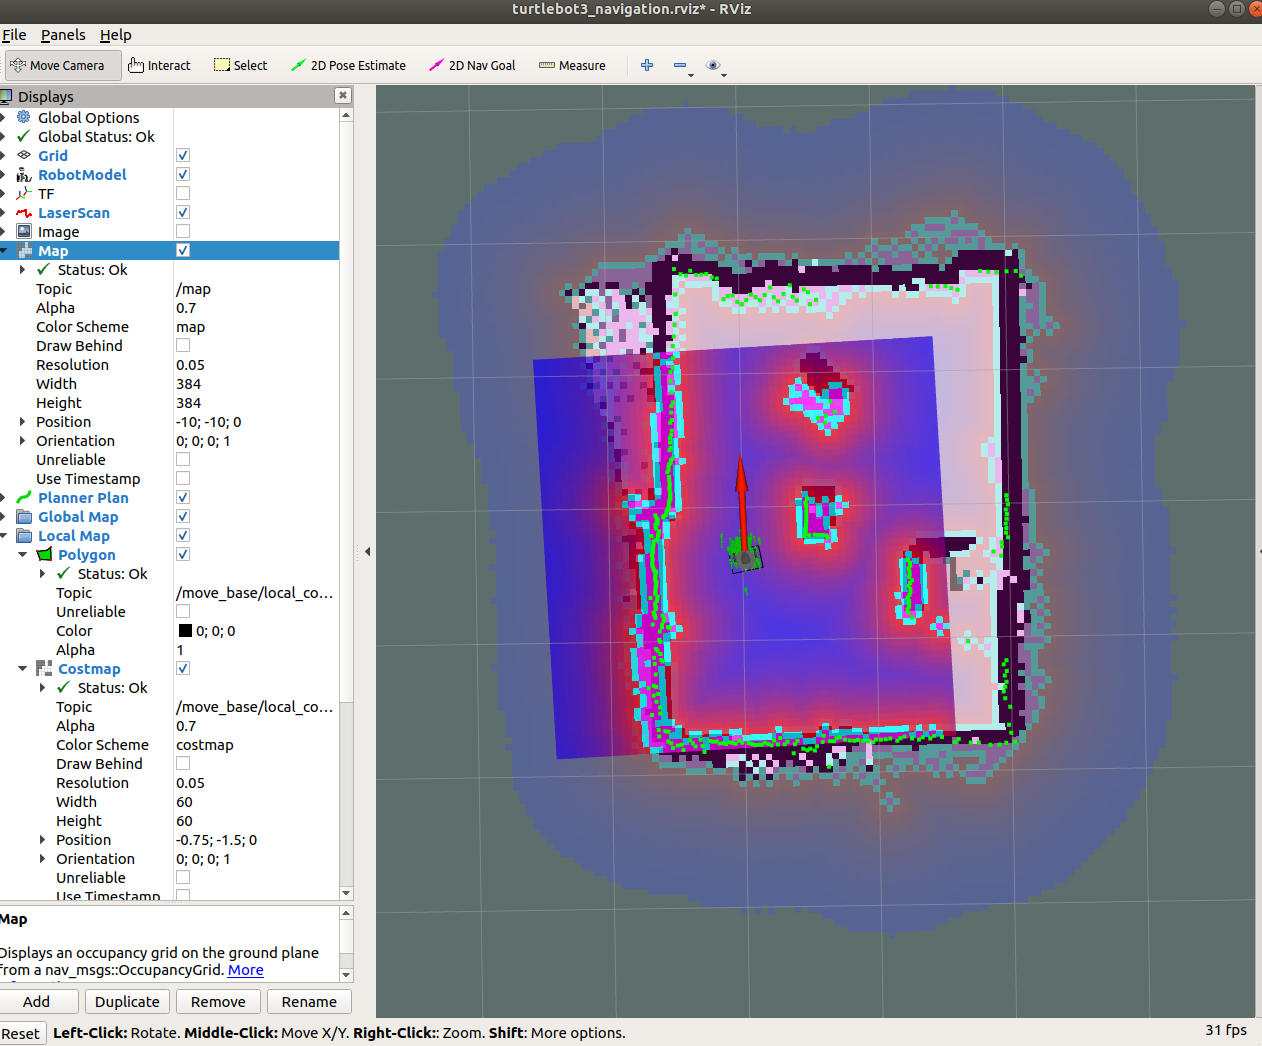
\includegraphics[width=1.0\linewidth]{figs/Rviz.png}
		\caption{Rviz}
		\label{Rviz}
	\end{center}
\end{figure}

実際に自律移動ロボットの研究を行う際は、PC上で表示している可視化した情報と現実空間を交互に見て比較を行う。
%@@@ちゃんと図に絡めて説明する。
しかし、この作業を行いながらロボットの追跡を行うのは面倒であり、現実空間での位置関係はイメージしづらい。
%@@@池邉君がかがんでいる写真を掲載しよう。https://www.youtube.com/watch?v=ObsD6C73Xr4 とか。

比較を手助けする技術の1つにAR(Augmented Reality)技術があげられる。
%@@@「あげられる」なので「1つに」じゃなくて「ひとつとして」かな?
ARとは、現実空間の映像にさまざまな情報を追加して表示する技術である。
自己位置推定の研究でもロボットが得た情報を現実空間に表示することで
交互に見るなどの作業を省くことで作業の効率化が見込められる。
また、比較の精度も可視化した情報が現実空間のどこに対応するのかイメージしながら行う従来の手法よりも高くなると考えられる。
ARを用いるメリットは、先行研究を踏まえて説明する。
%@@@これだけだとよくわからないので、あとで詳しく説明するとか書く。


\section{先行事例}

\subsection{AR ロボットコントローラ}
%%%%くっつけない!空行を入れる!!

ARを用いた比較を容易にする技術の先行事例として、
%@@@ちょっとどの言葉がどの言葉にかかるかよくわからない。
鈴木による「ARロボットコントローラ」\cite{鈴木勇矢2019ARロボットコントローラ}がある。
「ARロボットコントローラー」とは、画面上のタップした地点にロボットを自律移動させることができるアプリケーションである。
%@@@「このアプリケーションは、・・・できる。」くらいでよくない?くどい。
また、ロボットの操作と同時にロボットの内部情報も表示することができる。
図\ref{ARロボットコントローラー}にアプリケーションを実行している際の様子を示す。
図\ref{ARロボットコントローラー}では以下の情報を表示している。
\begin{itemize}
      \item 赤い丸:ロボットの初期位置
      \item 青い丸:目的位置
      \item 黒い線:移動経路
      \item 黄色い点 :Lidarのデータ
      \item 緑色の矢印:自己位置推定の結果のパーティクル
   \item ロボットを囲う赤い円:ロボットの位置姿勢
	%@@@これは図に書き込みましょうよ・・・
\end{itemize}
このアプリケーションで標示するパーティクルとは、モンテカルロ位置推定(以下MCL)によって推定したパーティクルである。
%@@@MCLの説明がない。「後述」でもいいので入れる。引用も。

\begin{figure}[H]
	\begin{center}
		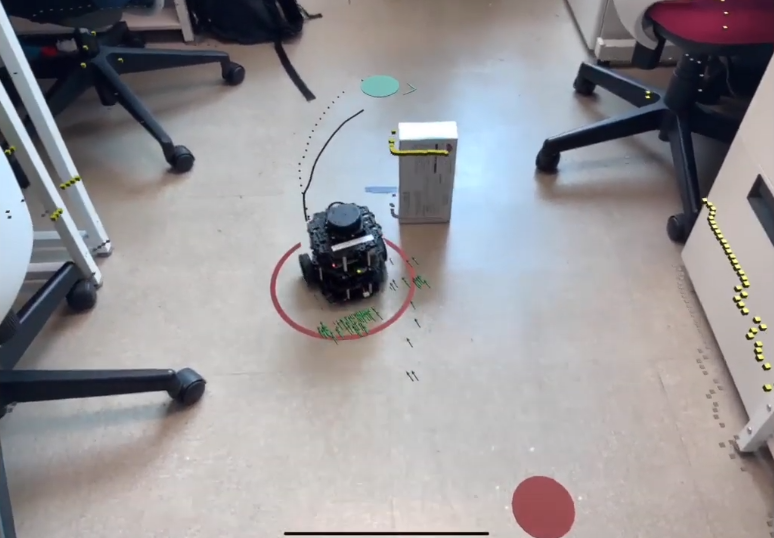
\includegraphics[width=1.0\linewidth]{figs/ARsuzuki.png}
		\caption{ARロボットコントローラー}
		\label{ARロボットコントローラー}
	\end{center}
\end{figure}
%画像

このアプリケーションのように、現実空間に内部情報を標示することで位置関係をイメージしやすくなる。
そのため、内部情報のデバックや評価もしやすくなると考えられる。

しかし、このアプリケーションの問題点として、一部の内部情報をアプリケーション上で正しく表示されないという問題点がある。
このアプリケーションでは、ロボットをオブジェクトとして認識し、ロボットがいる地点をパーティクルの中心と仮定してデータを表示している。
そのため、もしパーティクルがロボットから離れた位置を推定したとしても、パーティクルはロボットの周りに表示されてしまう。


\subsection{AR マーカーを用いた手法}

ARロボットコントローラの問題点を改善する手法として、高原によるARマーカーを用いる手法\cite{高原一樹2021ロボットの自己位置推定を可視化するAugmentedRealityアプリケーション}があげられる。
ARマーカーを用いる手法では、自己位置推定に用いるマップの原点にARマーカーを設置することで正しい位置に表示することを実現している。

しかし、ARマーカーを基準に表示を行うためARマーカーを見失ってしまうと表示しているデータの更新ができないという課題がある。
データの更新ができなくなる理由として、データを表示する際にARマーカーで座標を取得する必要があるためである。
そのため、ARマーカーを見失ってもアプリケーションを実行している端末が座標を推定する手段が必要だと考えられる。


\section{目的}

本研究では、マーカーレスで内部情報を表示するアプリケーションを開発する。
対象とする内部情報はLidarのデータである。


\section{論文構成}

論文構成

% dvipdfmxとhereのテスト
%\begin{figure}[H]
%	\begin{center}
%		\includegraphics[width=1.0\linewidth]{../zero.png}
%		\caption{}
%		\label{fig:}
%	\end{center}
%\end{figure}
%

%\include{purpose}
%\chapter{実現方法}\label{chap:method}

ARマーカーを用いずに原点を調整する手法として、マップ画像を用いて手動で調整する手法を提案する。


\section{内部情報の取得}

ロボットの内部情報の取得には、ROS#を用いた。
ROS#とは、Unity上でROSを利用できるようにするパケージで、UnityとROSでデータの通信が可能になる。
また、取得したデータは数値データであるため、可視化の作業もROS#を用いて行っている。
図\ref{VisRosUni}は、RvizとUnityでセンサーの可視化を行った様子である。
UnityでもRvizと同じような可視化結果が出力できていることがわかる。


\begin{figure}[H]
  \begin{minipage}[b]{0.45\linewidth}
    \centering
    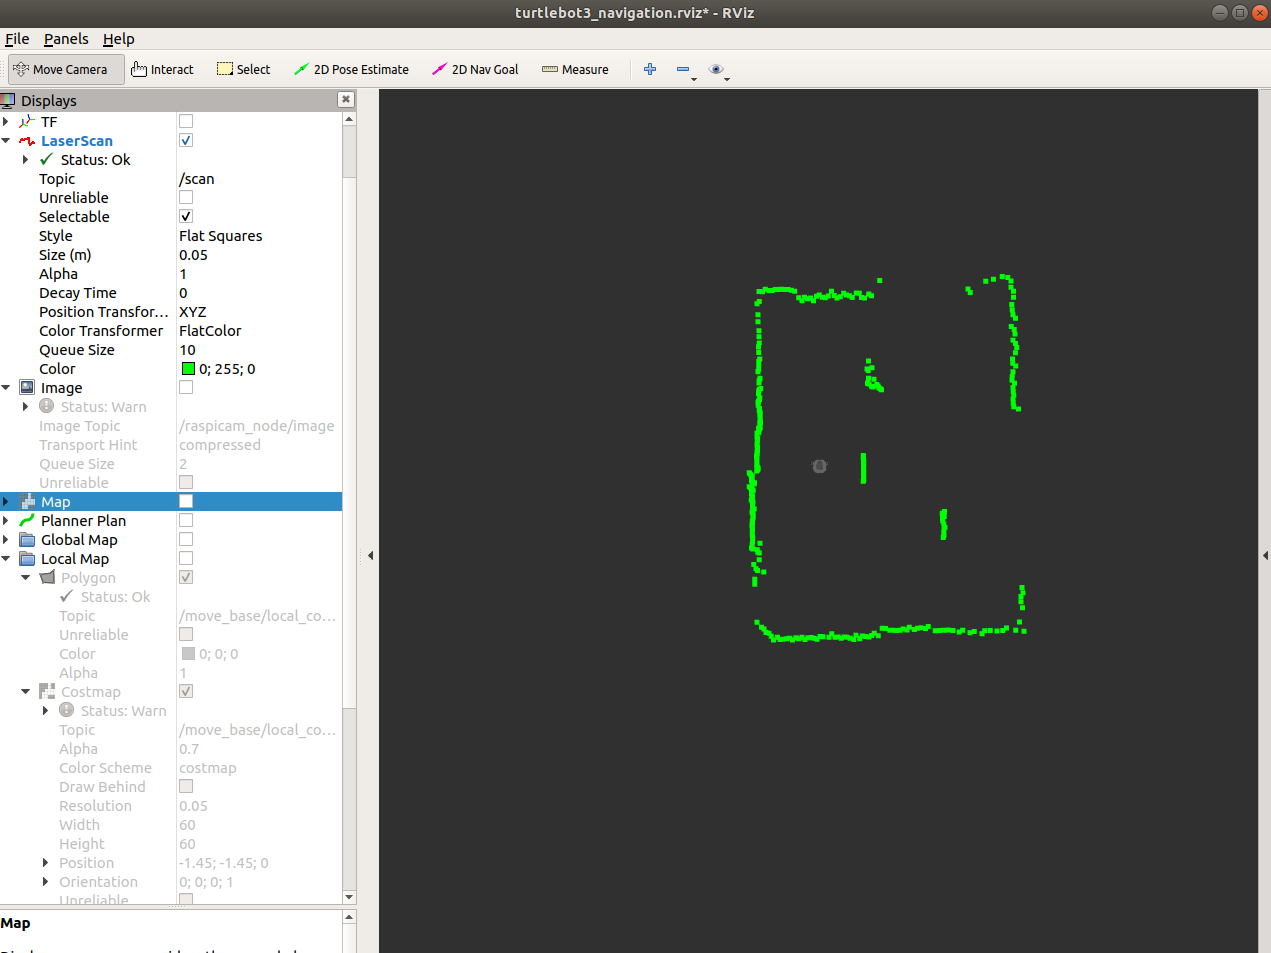
\includegraphics[keepaspectratio, width=.9\hsize]{figs/Rviz_Lidar.png}
    \subcaption{Rviz上での可視化}
  \end{minipage}
  \begin{minipage}[b]{0.45\linewidth}
    \centering
    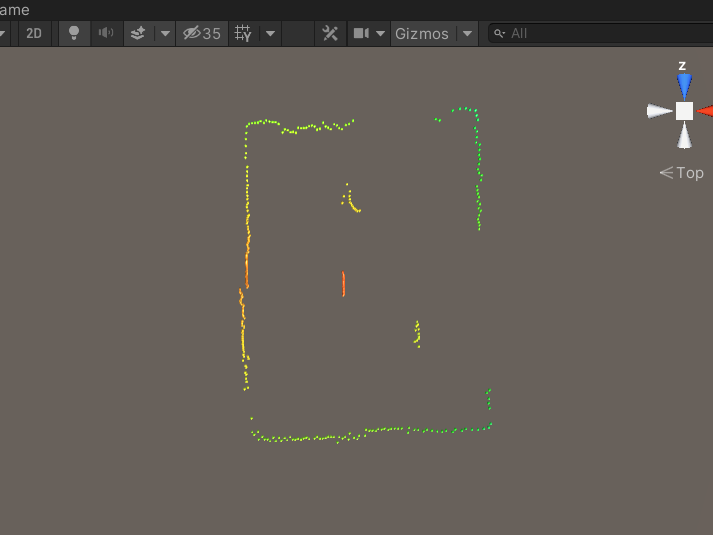
\includegraphics[keepaspectratio, width=.9\hsize]{figs/Unity_Lidar.png}
    \subcaption{Unity上での可視化}
  \end{minipage}
  \caption{データの可視化}\label{VisRosUni}
\end{figure}


\section{ARで可視化}

ARで可視化には、ARcoreを利用した。
ARcoreとは、Googleが提供するARプラットフォームであり、端末のトラッキングやオブジェクトの配置ができる。
トラッキングには、Visual Odometryという画像の特徴点から端末の移動量を推定する技術が利用されている。


\section{ARで可視化}


%\include{conclusion}

\appendix
\include{appendix}

%%% 参考文献 %%%
% よほどのことが無い限りet al.は使わないことにしましょう
\bibliographystyle{jualpha}
\bibliography{./references}

\newpage
\printindex

\end{document}
